\chapter{Text encoding}

\section{A brief history of character encoding}

\subsection{Bi-literal cipher of Francis Bacon}

In 1605, Francis Bacon, an English philosopher, scientist and statesman, devised the cipher that corresponds the English alphabete to a 5-bit code \cite{fbakoncipher}.

\begin{longtable}[H]{ c | c | c }
            Letter & Code & Binary \\
            \hline\hline
            A & aaaaa & 00000 \\
            B & aaaab & 00001 \\
            C & aaaba & 00010 \\
            & \dots & \dots \\
            F & aabab & 00101 \\
            & \dots & \dots \\
            L & ababa & 01010 \\
            & \dots & \dots \\
            Y & babba & 10110 \\
            Z & babbb & 10111 \\
            \hline
    \caption{Bacon's cipher}
\end{longtable}

The most powerful insight was that this cipher can be used for encoding by any two types of state: a pair of font style, "as by Bells, by Trumpets, by Lights and Torches, by the report of Muskets, and any inflruments of like nature".

Below is the example provided by Bacon. If a bold font syle denotes "a" and a normal font style denotes "b", then the phrase of 15 letters "Do not go til I come" can be transformed to:

\begin{figure}[t!]
    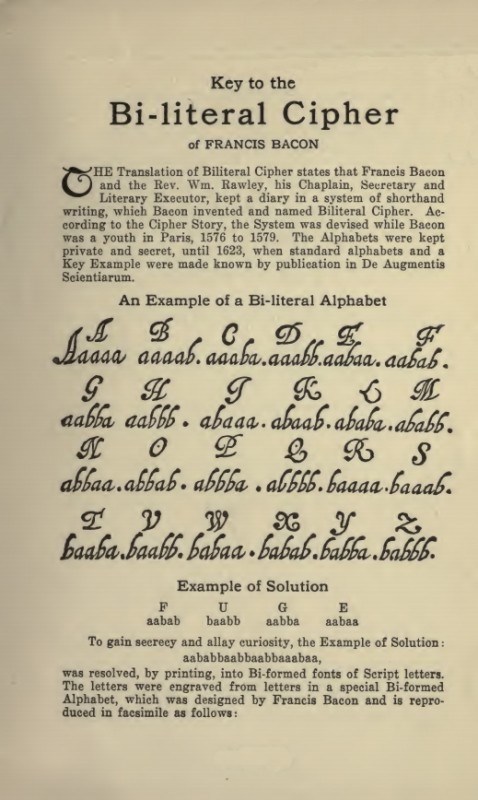
\includegraphics[width=\textwidth]{Bacon-cipher}
    \captionsetup{justification=centering,margin=1cm}
    \caption{Francis Bacon, Of the Proficience and Advancement of Learning, Divine and Human, 1605}
\end{figure}

\textit{\textbf{Do}} n\textit{\textbf{o}}t \textit{\textbf{g}}o \textit{\textbf{t}}i\textit{\textbf{l}} I \textit{\textbf{c}}ome 

$\downarrow$

aababababababba  

$\downarrow$ (group by 5)  

aabab ababa babba

$\downarrow$ (decode)

F L Y

In 1916, William Frederick Friedman, a US Army cryptographer, created an illustration how "anything can signify anything" with the Bacon's cipher \cite{fiedmanbaconcipher}.

\begin{figure}[h]
    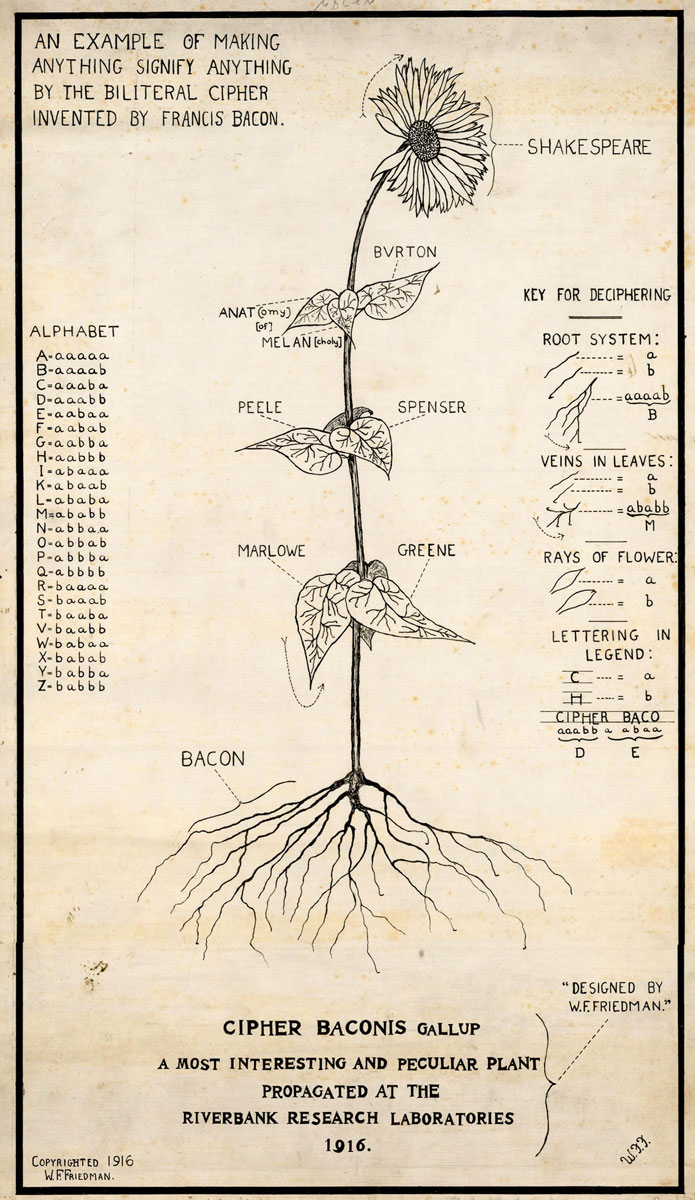
\includegraphics[width=\textwidth]{cabinet_040_sherman_william_h_002}
    \captionsetup{justification=centering,margin=1cm}
    \caption{W.F. Friedman, Cipher Baconis Gallup, 1916}
\end{figure}



\subsection{Gauss and Weber's code}

In 1833, Carl Friedrich Gauss and Wilhelm Weber, two German scientists, succeeded in transmitting messages via an electromagnetic data line at Gottingen Observatory. Although the invented telegraph had no financial funding and no further development, the variable 5-bit character code was invented \cite{martin2010technological}.

\begin{figure}[h]
    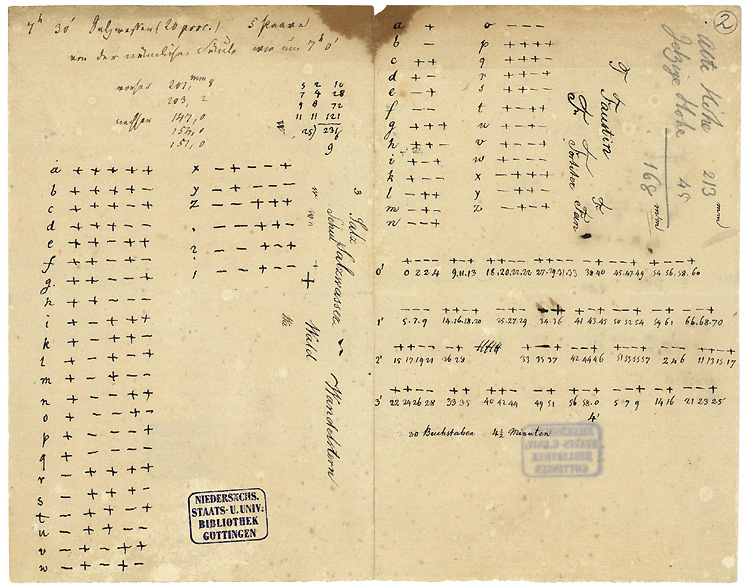
\includegraphics[width=\textwidth]{Gauss-Weber-code}
    \captionsetup{justification=centering,margin=1cm}
    \caption{Gauss and Webber's code, Göttingen University}
\end{figure}



\subsection{Morse and Gerke's code}

Samuel Morse invented the code for English alphabet, numbers and basic punctuations. In 1844, he send the first public American telegram from Washington to Ohio with the message "what hath God wrought?" ("what has God done?"). In the first version of Morse code each symbol is represented by a sequence of pulses of 4 length variants (base 4).

In 1848, Friedrich Gerke, a German writer, musician and telegraph technician, revised Morse's code. The new simplified version had a sequence of only a short and a long signal variants (base 2). Later, Gerke's code was adopted to International Morse-Gerke Code.

From the encoding perspective, we have the same pair of bits, now presented by the signal duration.

\begin{figure}[h]
    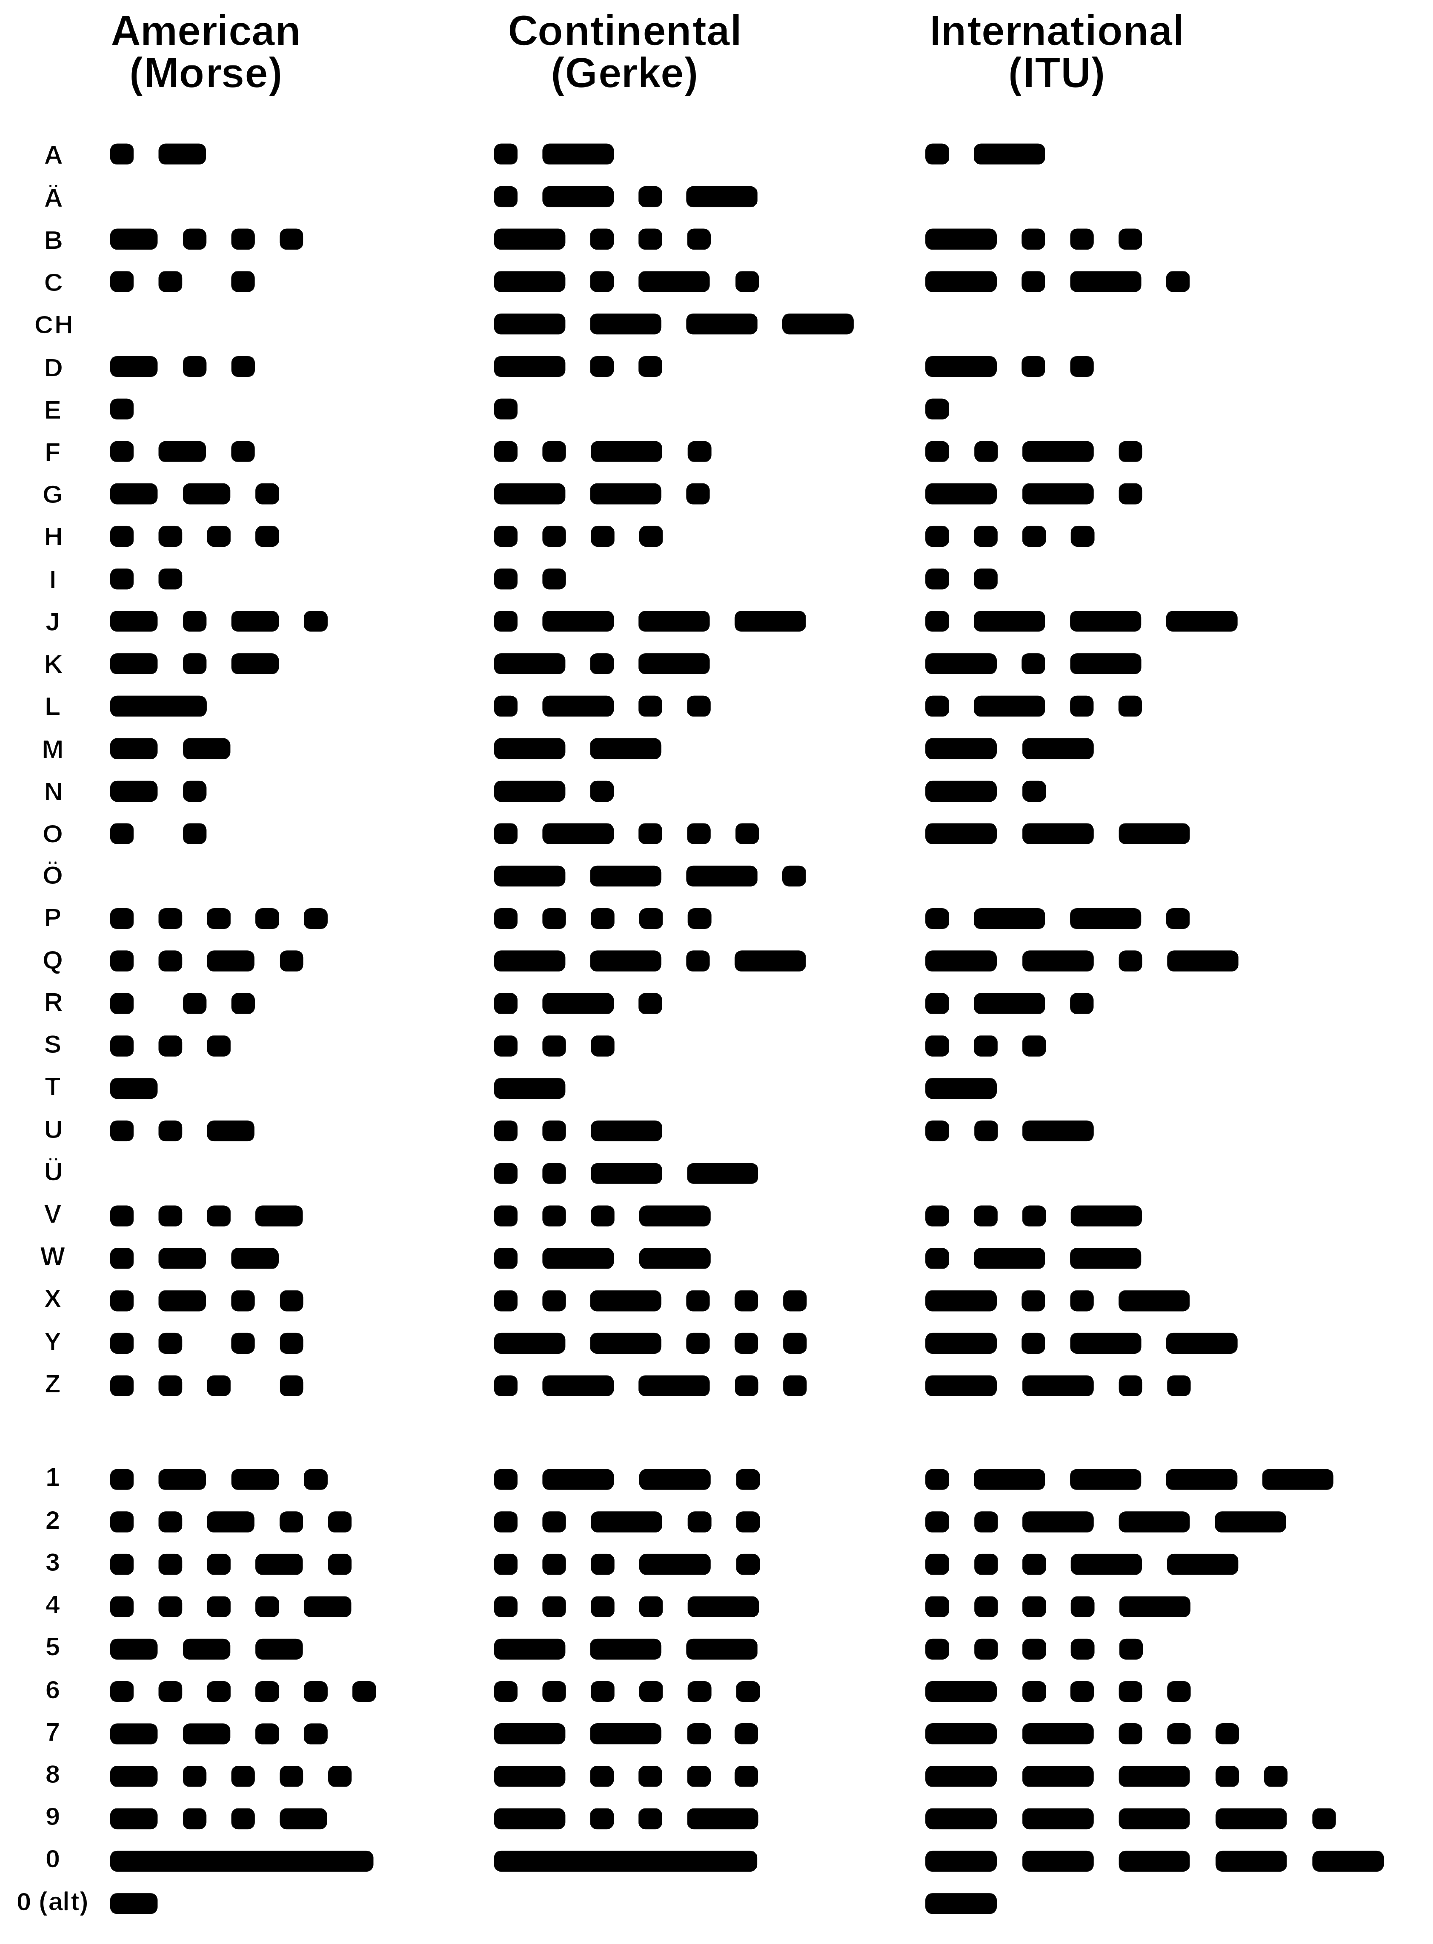
\includegraphics[width=\textwidth]{Morse_comparison}
    \captionsetup{justification=centering,margin=1cm}
    \caption{Morse, Gerke, ICU codes, Courtesy Spinningspark at Wikipedia}
\end{figure}

As an example, consider encoding of the famous emergency signal SOS that was introudced in the beginning of 20th century.

\begin{longtable}[H]{ c | c | c }
    S & O & S \\
    \hline
    ... & - - - & ... \\
    \hline
    000 & 111 & 000 \\
    \hline
    3 short & 3 long & 3 short \\
    \hline
\caption{SOS code}
\end{longtable}


\subsection{Baudot code}

In 1870s, Émile Baudot, a French telegraph engineer, invented a multiplex system for theleraph with the new 5-bit code for Roman alphabet, punctuation and control signals. The code was used in telegraph prior the ASCI